\section{Usability}
\label{sec:usability}
This chapter explains how to install and use the tool \Tool.

\subsection{Installation}
This section explains how to install the tool \Tool.
\begin{itemize}[leftmargin=*]
	\item Install a Python Interpreter (version 2.7 or 3).
				You may want to install a distribution (e.g. Python(x,y)) which already contains many useful packages.
	\item The tool \Tool will be delivered in a zipped folder \Code{Toro.zip}. 
				This folder has the following content:
				\begin{itemize}
				\item \textbf{Main script \Code{toro\_main.py}}, 
				\item \textbf{Libraries (pycpa, toro) in the folder \Code{libs}}.
				The libraries under \Code{./libs} are dynamically included. 
				They do not need to be installed unless you want to change their location.
				\item \textbf{Input folder \Code{data}.} Systems to be analyzed can be stored here.
				\end{itemize}
	\item Unzip the zip folder to your preferred destination.	
\end{itemize}


\subsection{Use}
This section gives an overview how to use the tool \Tool.
\begin{itemize}
\item Open a terminal and change to the \Code{/Toro} folder.	
\item The tool \Tool is called via the script \Code{toro\_main.py}.
A path is passed to the script as an argument to specify the location of the system to be analyzed.
It is recommended to store the system in the provided \Code{data} folder.
If several systems are to be analyzed, a subfolder can be created in \Code{data} for each system to be analyzed. 
The folder structure is illustrated in Figure \ref{fig:structure}.
\item An exemplary call of the tool would then look as follows:
\begin{tcolorbox}
\Code{\textbf{user@computer:\textasciitilde/Toro\$} python toro\_main.py ./data}
\end{tcolorbox}
%
\item The tool \Tool then executes, searching for specified systems. 
From the set of found systems, one ore more can interactively be selected for analysis.
Then the same procedure is repeated for each system to be analyzed:
\begin{itemize}
	\item User query to identify the type of system and verify assumptions about the system.
	\item Parsing the csv-files which specify the system (see Section \ref{sec:input-files}).
	\item Calculation of maximum end-to-end latencies and robustness margins.
	\item Generation of diagrams (see Section \ref{sec:output-files}). The files are written to the folder in which the analyzed system is specified.
	\item Creation of a file containing numerical results.  
	The file is written to the folder in which the analyzed system is specified.
\end{itemize}
\end{itemize}
%
\begin{figure}[t]
		\centering
				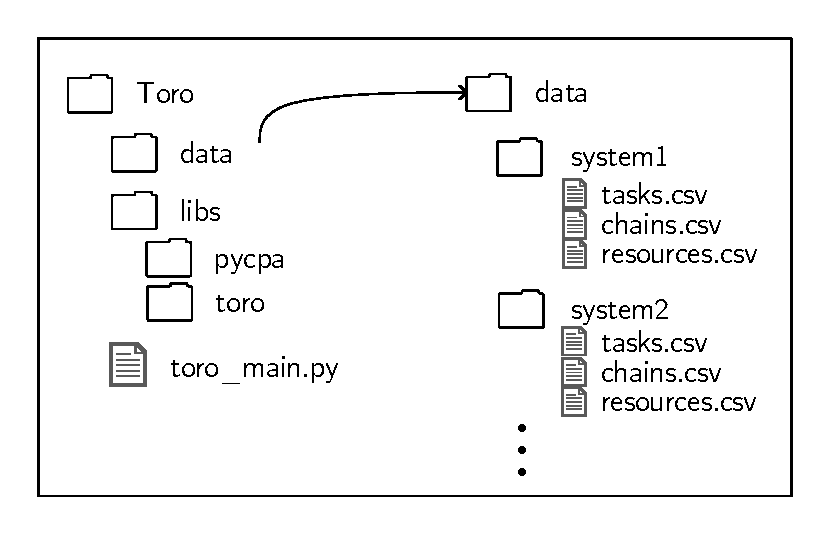
\includegraphics[trim=0.5cm 0.5cm 0.5cm 0.5cm, height=6cm]{fig/structure.pdf}
		\caption{Folder structure}
		\label{fig:structure}
\end{figure}
%


\subsection{Input Files}
\label{sec:input-files}
This section explains how to specify systems that the tool \Tool should analyze.
\bigskip

Firstly, \Tool calls the method \Code{get\_system\_dirs(dir)} and searches in the specified path for systems to be analyzed. 
Each individual system should be encapsulated in a dedicated folder as illustrated in Figure \ref{fig:structure}.
This system folder should contain three semicolon-separated csv-files, namely
\begin{itemize}[itemsep=0pt]
	\item \Code{chains.csv}, 
	\item \Code{resources.csv}, 
	\item \Code{tasks.csv}. 
\end{itemize}
These files can be created in Microsoft Excel, for example, and can then be exported as CSV files.
If \Tool finds more than one system in the specified top-level folder (e.g. \Code{.\textbackslash data}), the user can choose from a list which system(s) should be examined. 
An example output would look like this:
\begin{tcolorbox}
\small
{\Code{The following systems have been found:\\
\hspace*{15mm}1: system1\\
\hspace*{15mm}2: system2\\
\hspace*{15mm}2: system3\\
\hspace*{15mm}0: all\\
To select systems enter their ID or a comma-separated list of IDs. For instance, enter 1 to select the first of the listed systems, enter 1,3 to select the first and the third of the listed systems, or enter '0' to select all systems:}}
\end{tcolorbox}

The following sections \ref{sec:input-files-resources}-\ref{sec:input-files-chains} explain the structure of the CSV files. 
Then sections \ref{sec:input-files-bet1}-\ref{sec:input-files-let} demonstrate the three possible types of use cases and which information needs to be filled in.


\subsubsection{Input File 'resources.csv'}
\label{sec:input-files-resources}
The \Code{resources.csv} file describes the execution platform of the system by listing the different resources (CPUs, CAN bus etc.) and the scheduling policy that is applied on each resource. 
%Currently static priority preemptive and static priority non-preemptive scheduling is supported.
The \Code{resources.csv} file should have for each resource the following entries:
\begin{description}
		\item [name] Type: String \hfill \\ 
		Each computing core and each data bus, on which at least one chain task is executed, is represented by a so-called \emph{resource}.   This field specifies the name of the resource.		
		\item [scheduler] Type: String \hfill \\ 
		e.g., \Code{SPPScheduler} or \Code{SPNPScheduler}
\end{description}
\bigskip


\subsubsection{Input File 'tasks.csv'}
\label{sec:input-files-tasks}
The \Code{tasks.csv} file specifies tasks that are executed on the platform, it should have for each task the following entries:
\begin{description}
		\item [task\_name] Type: String \hfill \\ 
		Unique task ID
		\item [period] Type: Integer \hfill \\ 
		Activation period		
		\item [offset] Type: Integer \hfill \\ 
		Release offset
		\item [priority] Type: Integer \hfill \\ 
		Note that 0 is the highest priority.
		\item [wcet] Type: Integer \hfill \\ 
		Worst Case Execution Time		
		\item [resource] Type: String \hfill \\ 
		Resource that services the task. 
		The name should match a resource from file \Code{pycpa\_resources.csv}.
		\item [bcrt] Type: Integer \hfill \\ 
		Best Case Response Time		
		\item [wcrt] Type: Integer \hfill \\ 
		Worst Case Response Time
		\item [let] Typ: Integer \hfill \\ 
		Logical Execution Time 
\end{description}
\bigskip


\subsubsection{Input File 'chains.csv'}
\label{sec:input-files-chains}
The \Code{chains.csv} file specifies which tasks are part of each cause-effect chain; it should have for each chain the following entries:
\begin{description}
		\item [chain\_name] Type: String \hfill \\ 
		Unique cause-effect chain ID
		\item [e2e\_deadline] Type: Integer \hfill \\ 
		End-to-end deadline 		
		\item [members] Type: String \hfill \\ 
		The member tasks must be listed in correct order and the task names must match those in the task definitions. The list of member tasks comprises as many cells in a row as needed.
\end{description}



\newpage
\subsubsection{Use Case 1: Cause-effect chains with BET tasks, WCRT for each chain task known}
\label{sec:input-files-bet1}

\begin{tcolorbox}
\begin{itemize}[leftmargin=*, itemsep=0pt]
	\item applicable to many systems
	\item the name, period, offset, WCRT of every task in a cause-effect chain must be known
\end{itemize}
\end{tcolorbox}
\bigskip

\emph{Use Case 1} requires that
\begin{itemize}[leftmargin=*, itemsep=0pt]
	\item all clocks in the system are synchronized,
	\item all tasks in the cause-effect chains are BET tasks,
	\item task deadlines are implicit,
	\item all BCRTs and WCRTs of chain tasks are known,
\end{itemize}
which is checked in an interactive user query.
\bigskip

An example system of type \emph{Use Case 1} is depicted in Figure \ref{fig:use-case-1}.
For the example system, the file \Code{resources.csv} would contain:
\begin{center}
	\begin{tabular}{|l|l|} \hline
		\textbf{name} & \textbf{scheduler} \\ \hline
		unknown & unknown \\ \hline
	\end{tabular}
\end{center}
With regard to the tasks that are part of the cause-effect chains to be analyzed, we have in \Code{tasks.csv} 
\begin{center}
	\begin{tabular}{|l|l|l|l|l|l|l|l|l|} \hline
		  \textbf{task\_name}  
		& \textbf{period} 
		& \textbf{offset} 
		& \textbf{priority}
		& \textbf{wcet}
		& \textbf{resource} 
		& \textbf{bcrt}		
		& \textbf{wcrt}
		& \textbf{let} \\ \hline
		BET\_T1&10&2&n/a&n/a&unknown&0&5&n/a \\ \hline
		BET\_T4&20&5&n/a&n/a&unknown&2&15&n/a \\ \hline 
		BET\_T5&5&0&n/a&n/a&unknown&1&3&n/a \\ \hline
		BET\_T7&15&1&n/a&n/a&unknown&3&10&n/a \\ \hline
		BET\_T9&30&5&n/a&n/a&unknown&5&20&n/a	\\ \hline	
	\end{tabular}
\end{center}
Note that a number of fields in \Code{resources.csv} and \Code{tasks.csv} can be declared as 'unknown' resp. 'n/a' because the WCRTs are already available and do not need to be computed from these parameters.
\bigskip

The cause-effect chains in \Code{chains.csv} are specified by
\begin{center}
	\begin{tabular}{|l|l|l|l|l|l|} \hline
		\textbf{chain\_name} 
		& \textbf{e2e\_deadline}
		& \multicolumn{4}{|l|}{\textbf{members}} \\ \hline
			BETchain1 & 75 & BET\_T1 & BET\_T5 & BET\_T7 & BET\_T9 \\ \hline
			BETchain2 & 40 & BET\_T4 & BET\_T1 & & \\ \hline
	\end{tabular}
\end{center}
%
\begin{figure}[h!]
	\centering
		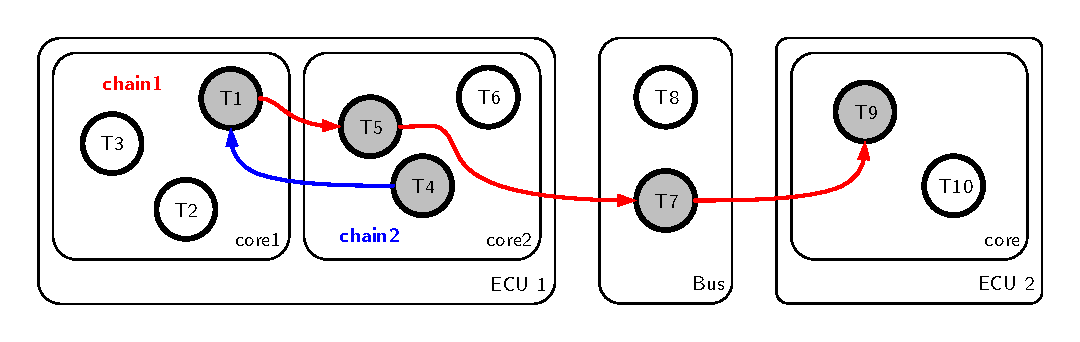
\includegraphics[height=4cm, trim = 0.5cm 0.5cm 0.5cm 0.5cm]{fig/bet1-system.pdf}
	\caption{\emph{Use Case 1}. Parts of the system, which are relevant for the analysis, are shaded.}
	\label{fig:use-case-1}
\end{figure}



\subsubsection{Use Case 2: Cause-effect chains with BET tasks,\\ WCRT of each chain task computable}
\label{sec:input-files-bet2}

\begin{tcolorbox}
\begin{itemize}[leftmargin=*, itemsep=0pt]
	\item only applicable to systems with \ac{spp} und \ac{spnp} scheduling
	\item not only tasks that are part of cause-effect chains must be specified but also the entire background load with all parameters
\end{itemize}
\end{tcolorbox}

\emph{Use Case 2} requires that
\begin{itemize}[leftmargin=*, itemsep=0pt]
	\item all clocks in the system are synchronized,
	\item ALL tasks are BET tasks (not only those in the listed cause-effect chains),
	\item task deadlines are implicit,	
	\item task offsets are zero,
	\item ALL tasks in the system must be known with their parameters,
	\item ALL resources must be known with their scheduling algorithms (SPP or SPNP) and the task-to-resource mapping,
\end{itemize}
which is checked in an interactive user query.
\bigskip


An example system of type \emph{Use Case 2} is depicted in Figure \ref{fig:use-case-2}.
For the example system, the file \Code{resources.csv} would contain:

\begin{center}
\small
	\begin{tabular}{|l|l|} \hline
		\textbf{Name} & \textbf{Scheduler} \\ \hline	
		core\_1 & sppscheduler \\ \hline	
		core\_2 & spnpscheduler	\\ \hline		
	\end{tabular}
\end{center}

With regard to the tasks that are part of the cause-effect chains to be analyzed, we have not only the chain tasks but also the tasks of the background load with all parameters required to compute the WCRTs.
\begin{center}
	\begin{tabular}{|l|l|l|l|l|l|l|l|l|} \hline
		  \textbf{task\_name}  
		& \textbf{period} 
		& \textbf{offset} 
		& \textbf{priority}
		& \textbf{wcet}
		& \textbf{resource} 
		& \textbf{bcrt}		
		& \textbf{wcrt}
		& \textbf{let} \\ \hline
			BET\_T1&5&0&1&1&core\_1&n/a&n/a&n/a \\ \hline
			BET\_T3&15&0&3&3&core\_1&n/a&n/a&n/a \\ \hline
			BET\_T5&10&0&2&2&core\_1&n/a&n/a&n/a \\ \hline
			BET\_T2&10&0&2&1&core\_2&n/a&n/a&n/a \\ \hline
			BET\_T4&5&0&1&1&core\_2&n/a&n/a&n/a \\ \hline
			BET\_T6&20&0&3&4&core\_2&n/a&n/a&n/a \\ \hline
	\end{tabular}
\end{center}

The cause-effect chains are specified again by
\begin{center}
	\begin{tabular}{|l|l|l|l|l|l|} \hline
		\textbf{chain\_name} 
		& \textbf{e2e\_deadline}
		& \multicolumn{3}{|l|}{\textbf{members}} \\ \hline
			BETchain1 & 50  & BET\_T1 & BET\_T3 & BET\_T2 \\ \hline
			BETchain2 & n/a & BET\_T1 & BET\_T4 & \\ \hline
	\end{tabular}
\end{center}
%
\begin{figure}[h!]
	\centering
		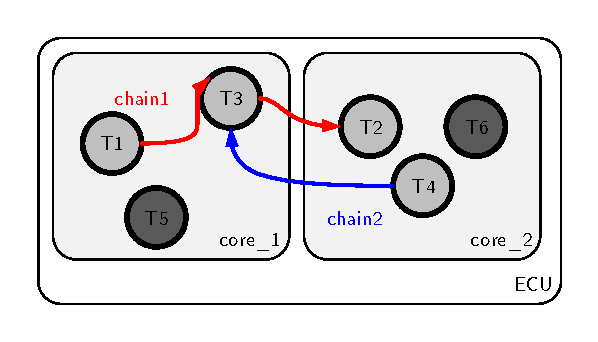
\includegraphics[height=4cm, trim = 0.5cm 0.5cm 0.5cm 0.5cm]{fig/bet2-system.pdf}
	\caption{\emph{Use Case 2}. Parts of the system, which are relevant for the analysis, are shaded.}
	\label{fig:use-case-2}
\end{figure}



\subsubsection{Use Case 3: Cause-effect chains with LET tasks, LET for each chain task known}
\label{sec:input-files-let}
%
\begin{tcolorbox}
\begin{itemize}[leftmargin=*, itemsep=0pt]
	\item applicable to LET systems
\end{itemize}
\end{tcolorbox}
\bigskip

\emph{Use Case 3} requires that
\begin{itemize}[leftmargin=*, itemsep=0pt]
	\item all clocks in the system are synchronized,
	\item all tasks in the cause-effect chains are LET tasks,
	\item all LET tasks have implicit deadlines,	
\end{itemize}
which is checked in an interactive user query.
\bigskip

An example system of type \emph{Use Case 3} is depicted in Figure \ref{fig:use-case-3}.
For the example system, the file \Code{resources.csv} would contain:
\begin{center}
	\begin{tabular}{|l|l|} \hline
		\textbf{name} & \textbf{scheduler} \\ \hline
		unknown & unknown \\ \hline
	\end{tabular}
\end{center}
With regard to the tasks that are part of the cause-effect chains to be analyzed, we have in \Code{tasks.csv} 
\begin{center}
	\begin{tabular}{|l|l|l|l|l|l|l|l|l|} \hline
		  \textbf{task\_name}  
		& \textbf{period} 
		& \textbf{offset} 
		& \textbf{priority}
		& \textbf{wcet}
		& \textbf{resource} 
		& \textbf{bcrt}		
		& \textbf{wcrt}
		& \textbf{let} \\ \hline
	LET\_T1&10&2&n/a&n/a&unknown&n/a&n/a&5 \\ \hline
	LET\_T4&20&5&n/a&n/a&unknown&n/a&n/a&15 \\ \hline
	LET\_T5&15&1&n/a&n/a&unknown&n/a&n/a&10 \\ \hline
	LET\_T7&5&0&n/a&n/a&unknown&n/a&n/a&3 \\ \hline
	LET\_T9&10&1&n/a&n/a&unknown&n/a&n/a&5 \\ \hline		
	\end{tabular}
\end{center}

The cause-effect chains are specified by
\begin{center}
	\begin{tabular}{|l|l|l|l|l|l|} \hline
		\textbf{chain\_name} 
		& \textbf{e2e\_deadline}
		& \multicolumn{4}{|l|}{\textbf{members}} \\ \hline	
		LETchain1 & 45 &LET\_T1 &LET\_T5 &LET\_T7 &LET\_T9 \\ \hline	
		LETchain2 & 35 &LET\_T4 &LET\_T1 & &\\ \hline			 
	\end{tabular}
\end{center}
%
\begin{figure}[h!]
	\centering
		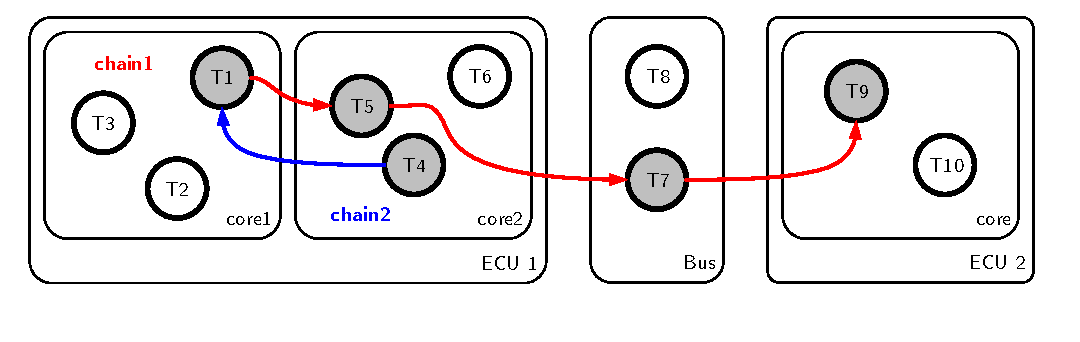
\includegraphics[height=4cm, trim = 0.5cm 0.5cm 0.5cm 0.5cm]{fig/let-system.pdf}
	\caption{Use case 3. Parts of the system, which are relevant for the analysis, are shaded.}
	\label{fig:use-case-3}
\end{figure}
\FloatBarrier
\hfill
\pagebreak[4]


\newpage
\subsection{Output Files}
\label{sec:output-files}
Outputs are written into the folder of the specified system.

\subsubsection{Log File}
The numberical results are written to the text file 
\Code{RESULTS\_LOG.txt}.

\subsubsection{Interval Diagram}
In the interval diagram, the individual jobs are represented as numbered circles. 
The blue-marked read intervals represent the earliest possible to latest possible time, when a job can read data. 
The green-marked data intervals bound the period of time in which the output data of a job is available to other jobs.
The short vertical lines stand for the period of a task.
The long vertical lines show the hyper period (HP).
\smallskip

The yellow area covers all instances of the cause-effect chain which are relevant for the computation of the maximum end-to-end latency and the robustness margins. \\
The dark area highlights one instance of a cause-effect chains which actually has the maximum end-to-end latency. \\
The red areas illustrate some selected robustness margins, which are valid for the isolated cause-effect chain and guarantee the end-to-end deadline (type 2 of a robustness margin, see Section \ref{sec:robustness-margins}).
%
\begin{figure}[h!]
		\centering
		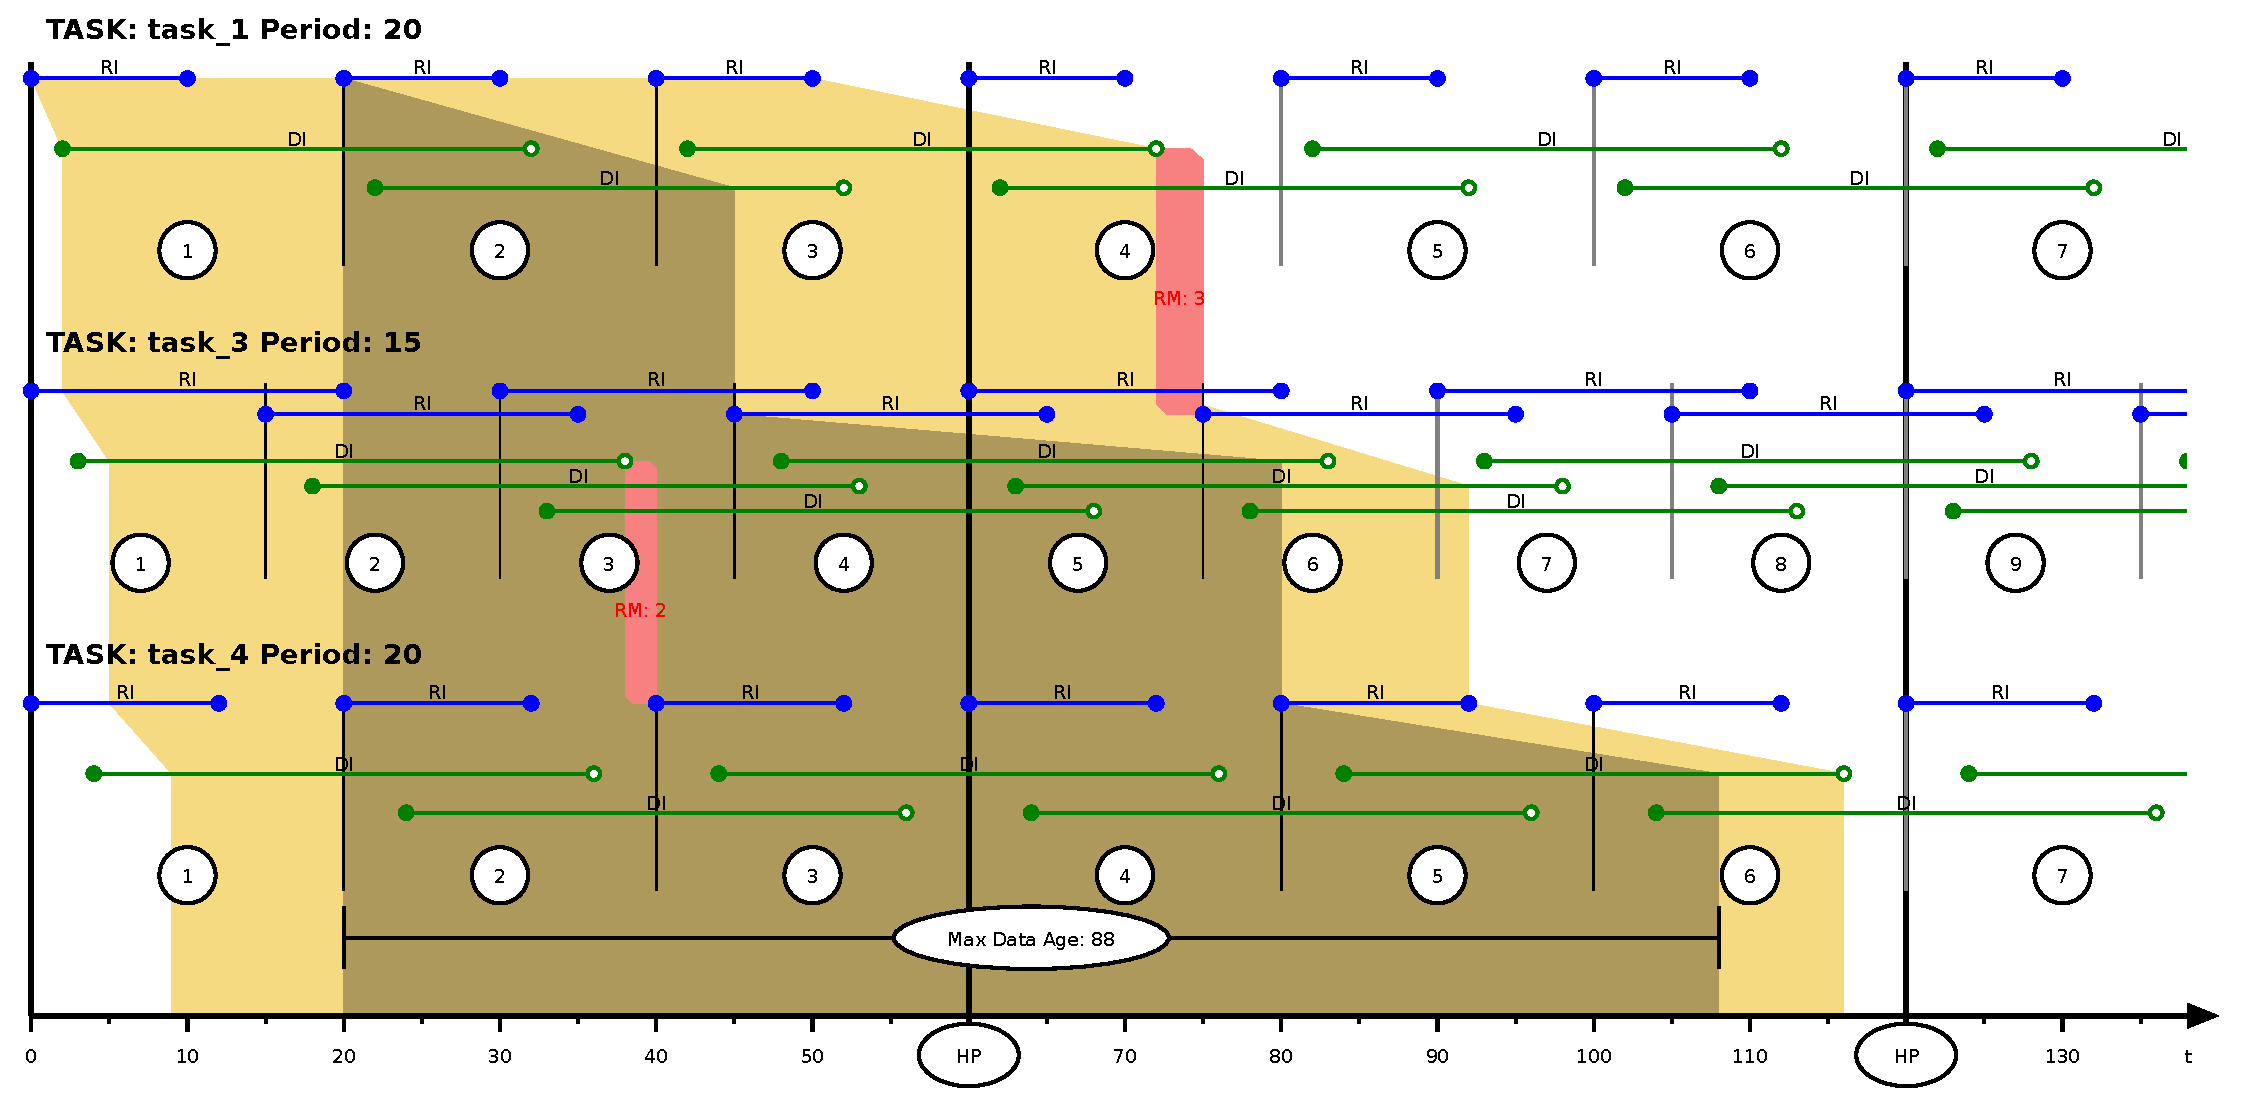
\includegraphics[width=415pt]{fig/intervalls.pdf}
		\caption{Interval diagram.}
		\label{fig:interval_diagram}
\end{figure}


\newpage
\subsubsection{Reachability Graph}
%
\begin{figure}[H]
		\centering
		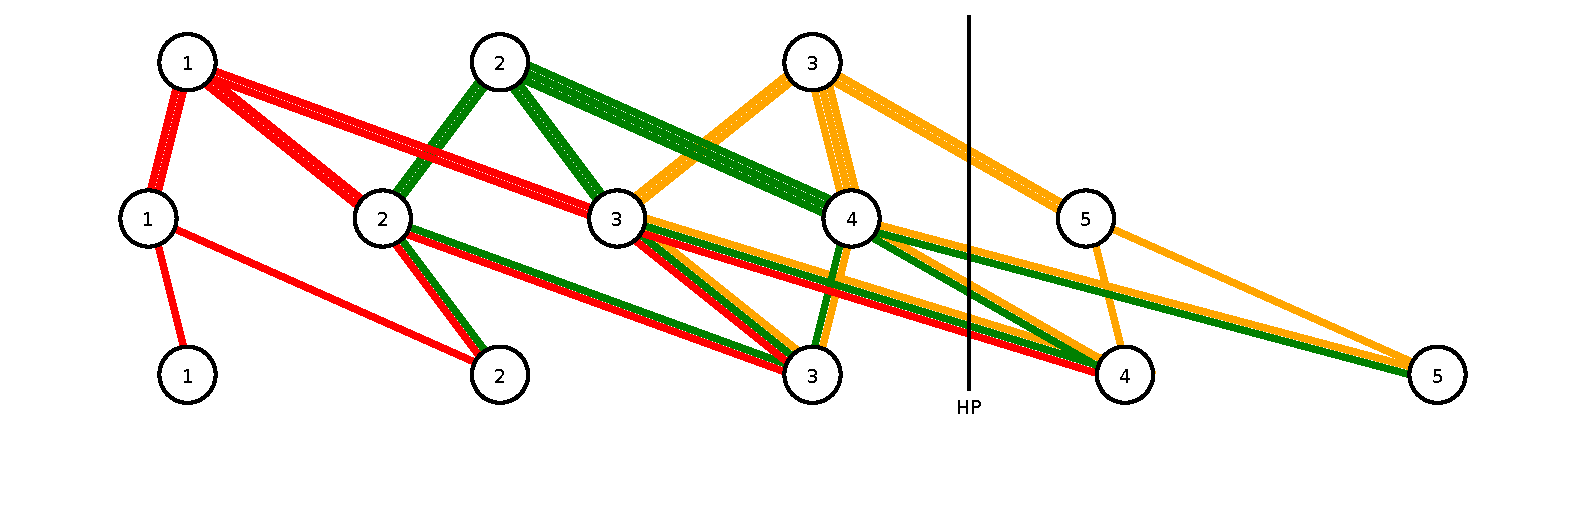
\includegraphics[width=400pt]{fig/tree.pdf}
		\caption{Reachability graph}
		\label{fig:reachability}
\end{figure}
%
The reachability graph results from the overlap of read intervals and data intervals of jobs (data flow analysis). 
In the reachability graph, all possible paths of starting in from the first hyperperiod are represented.
These paths are required for the computation of the maximum end-to-end latency and the robustness margins. 
The colored marking of the individual paths makes it easy to recognize where a path begins and ends. The numbers stand for the respective job number. 
    

\newpage
\subsubsection{Overview Graph}
The overview graph represents the specified cause-effect chains as a tasks with data flow dependencies.

%
\begin{figure}[H]
  \centering
  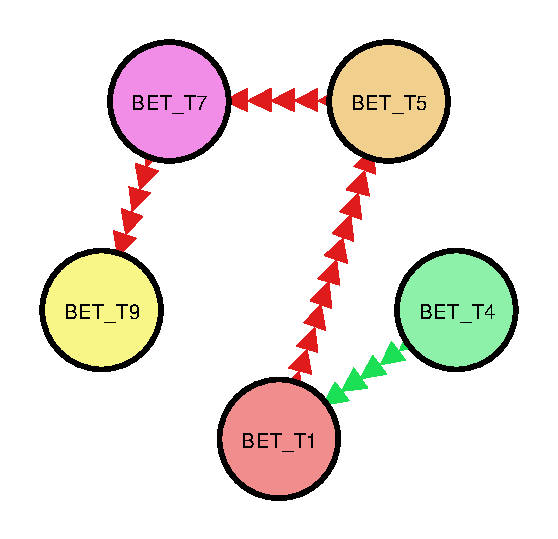
\includegraphics[width=0.7\textwidth]{fig/results.pdf}
  \caption{Overview graph}
  \label{fig:summ_diagram}
\end{figure}
